%!TEX root = ../thesis.tex

%%%%%%%%%%%%%%%%%%%%%%%%%%%%%%%%%%%
%    BEYOND THE STANDARD MODEL    %
%%%%%%%%%%%%%%%%%%%%%%%%%%%%%%%%%%%

%\newchap{Theoretical Motivations}
\message{^^J ^^J BEYOND THE STANDARD MODEL ^^J ^^J} % print to log
\newchap{Beyond the Standard Model}\label{sec:BSM}

The SM of particle physics is successful.
Fine-structure constant $\alpha=e^2/4\pi$ has been precisely calculated and measured~\cite{g-2_e_theory1,g-2_e_theory2,g-2_e_theory3,g-2_e_Cambridge1}.
In 2012, the discovery of the Higgs boson was announced by the ATLAS and CMS experiments at the CERN LHC~\cite{Higgs_discovery_2012_CMS,Higgs_discovery_2012_ATLAS,Higgs_discovery_2013_CMS,Higgs_mass_2015_combined}, more than 47 years after its prediction~\cite{Higgs_theory1,Higgs_theory2}.
But there are both problems.
The following section highlights several examples of open questions in physics.

% FIGURE: SCALE
%!TEX root = ../thesis.tex

% FIGURE: energy scale
\begin{figure*}[t]
  %\vspace{-12mm}
  \centering
  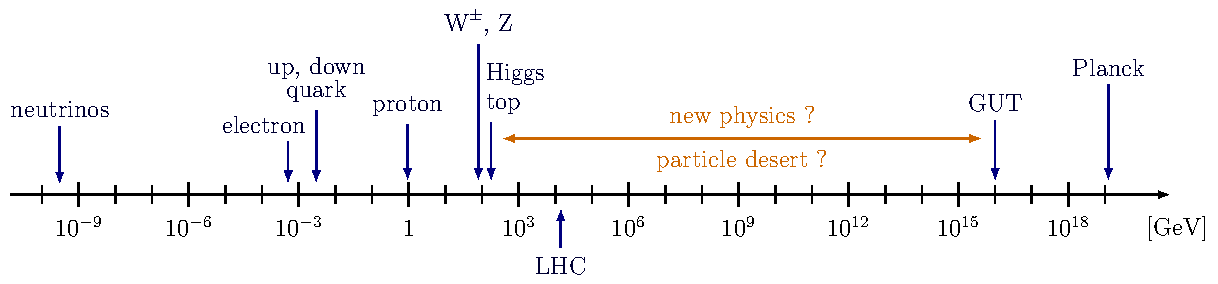
\includegraphics[width=1.02\textwidth]{fig/intro/SM_timeline.pdf}
  \vspace{-3mm}
  \caption{
Logarithmic scale of different energy scales in particle physics.
Adapted from Ref.~\cite{particle_physics_timeline_fig}.
  } \label{fig:energy_scales}
  %\vspace*{-3mm}
\end{figure*}

